\documentclass{article}

\usepackage[utf8]{inputenc}
\usepackage[left=1.5in,right=1.5in,bottom=1in]{geometry}
\setlength\parindent{0pt}
\setlength{\parskip}{1em}
\setcounter{secnumdepth}{0}
\usepackage{outlines}
\usepackage{graphicx}
\graphicspath{ {imgs} }

\title{Urban Economic Geography}
\author{Carla Hyenne }

\begin{document}

\maketitle

\tableofcontents

\pagebreak

% LECTURE 1

\section{The City as a Social Product}
\date{September 30th, 2021}

There is no such thing as a "pure", "neutral" knowledge or definition of cities/urban space. There are empirical observations, like the density, retail, urban projects, transport, road safety regulations, etc. However, what we see isn't enough. We need concepts, theories, models, abstract tools to make sense of the city.

The type of "intellectual" glasses that we wear influence what and how we understand the space and the issues within it. For example in economics, your views change if you are wearing capitalist vs. socialist glasses.

Thus, what epistemological choices is this class based on? It takes distance from the "urban triumphalism" mainstream, and takes a critical stance on urban issues. 

\subsection{Urban Triumphalism}

Triumphalism depicts cities as a site of progress, a way to prosperity, and we are in a "golden age" of the city. The major \textbf{contemporary challenges} are first urban challenges, and the urban space is where \textbf{solutions} are found. Think of the green, smart, productive, participative, etc., city. 

The key question is then \textit{how} to re-organise the city in order to meet these challenges, by using the potentialities and opportunities in the urban environment. 

\subsubsection{What is the problem with urban triumphalism?}

\begin{outline}
  \1 Urban triumphalism is purely a pro-growth perspective, which is contradictory with the sustainability targets (continuous growth is not sustainable). 
  \1 It is only about finding solutions to a series of pre-defined challenges: how to build the city, equip the city, govern the city, brand the city... This turns urban issues into \textbf{techno-management} issues, where the focus in on the best practices that can be copy/pasted, and where the focus is: 
  \2 on city leaders' views, 
  \2 on best practices for copy/pasting solutions, and 
  \2 on mass production of city rankings which highlight competition

  \1 Consultancy firms (McKinsey) are now targeting the 'CEOs' of cities, that is the mayors, to propose techno-managerial solutions to urban problems. 
These firms are usually focused on maintaining the \textbf{competitiveness} of cities, so that the livelihoods of residents are maintained. This statement from McKinsey is contradictory, since most residents are not involved in making the city competitive, and could be better off if cities were less capitalist.

The mass production of city rankings, also done by consultancy firms, are not transparent. They emphasise the importance of competition amongst cities

  \1 There is a strong inclination towards \textbf{reification} (treating something immaterial, as a material thing). 
  	\2 The social objects are conceived as a mere thing, a coherent and active whole. Cities are viewed as actors
	\2 The city is viewed as an actor ("the city does this"), and acts according to a series of shared interests and aspirations. However, what is good for one is not always good for the other (usually, what's good for businesses/elites is not good for the rest) 
\end{outline}

Marcuse, in \textit{The City as a Perverse Metaphor} explains that seeing the city as an actor excludes a set of the population who does not share the same interests and aspirations. Not all the city is international, competitive, and so on, even if some firms, some people might be. 

\subsubsection{Breaking with Triumphalism}

\begin{outline}
	\1 The city is not an actor, but a \textbf{dynamic space} where actors with different resources, interests, aspirations, interact in diverse ways, from open conflict violence to resistance, mobilisation, collaboration, solidarity
	\1 Urban issues are not all \textbf{techno-managerial} ones, but also \textbf{political}
		\2 Urban space are composed of an established web of social relations, sedimented through history in a specific geographical context
		\2 Urban change is therefore fundamentally conflictual, regarding material forms, norms, regulations, symbolic landscapes... (these are political conflicts, where disagreement and lack of consensus is the default)
		\2 Thus, \textbf{urban landscapes are dynamic and contested landscapes of social power}\footnote{Example: the Berlin referendum on collectivisation, to decide who decides on the rent of the city. This shows the politicisation of an urban space, where a group of individuals use their social power to contest regulations.}
\end{outline}

\subsection{Critical urban studies}

\subsubsection{Definition}

Critical urban studies are
\begin{outline}
	\1 Contra \textbf{naturalising} views: there is nothing natural about cities, how they are shaped, built, transformed, governed, represented. They are not a "living organism"
	\1 Contra \textbf{techno-managerial} takes on urban issues: focus instead on tensions and contradictions, and not solutions to standardised challenges
\end{outline}

Cities are not permanent, but \textbf{dynamic force fields, shaped by social forces, acting through complex set of actors embedded in historically and geographically situated configurations of power relationships.}

Critical urbanism started in the 1960's in the US, because the existing theoretical frameworks could not explain what was happening on the streets:

\begin{outline} 
	\1 Detroit 1967: 1967 Detroit riots, confrontation of black residents and Detroit police)\footnote{"Social Justice and the City", David Harvey} 
	\1 Bruxelles 1969: La Marolle protest, by residents against plans to expand the justice palace into the Marolle quartier 
\end{outline}

\subsection{The production of urban space}

Urban space can, and has been, produced differently. It often gives insights in to the type of society who lived there

\begin{outline}
	\1 Hierarchical society: Nuremberg 15th century. A castle with a moat suggest feudal society, the city walls suggest a violent society
	\1 Agricultural, centralised, rural society: fictional rendition of Babylon, the power is concentrated in a city within the city
	\1 Colonial society: Santiago de Chile, 16th century. The grid guidelines typical of Spanish colonial development
	\1 Industrial society: Roubaix, 20th century. Villes-cheminées (stacks), where work, home, leisure spaces were in the same place\footnote{Friedrich Engels, "The Condition of the Working Class in England"}
\end{outline}

In each society, spatial configurations are organised a specific, non-arbitrary ways, in the image and in support of a particular \textbf{social order}. A soviet (or post-soviet) city, with large boulevard/impressive and brutalist architecture is organised differently from capitalist American cities.

For any society at different moments in time, ordering its space (material, function, political-administrative, symbolic dimensions) is as crucial as organising its production system, its political/legal framework, its cultural/ideological/estethic norms...

\subsubsection{Production of space today}

What picture should we paint to describe the society of today? Landscapes of skyscrapers, or slums and inequality, private or public space (or privatised public space?), of consumption, blurred boundaries, planetary dimensions, transportation and networks?

There are many landscapes: skyscrapers of Doha, skyscrapers vs. disinvested neighbourhoods of Detroit showing sharp inequalities, the ultra libertarian and capitalist Space X with no state regulation.

\subsubsection{Heuristic of the production of urban space}

\begin{outline}
	\1 Move \textbf{from an essentialist, to a relational thinking} about cities. Cities do not have a set of attributes that are necessary for them to "a  city". The object is not 'the city', but the dynamic relationships of societies to urban space. 
	\\\textit{Relational thinking: cities as social products}
	\1 Move \textbf{from a historical to a diachronic thinking} about cities. The production of space is always a "work in progress", through which inherited socio-spatial configurations are reshaped according to new logics. That is, the urban spaces in a \textit{permanent flow of creative destruction}
	\\\textit{Diachronic thinking: cities as "work in progress"}
	\2 Examples of impermanent, in progress urban landscapes: 
		\3 Place De Brouckère, Brussels: project to remove traffic from the boulevard, and undo the work from the 60s where axes of transit (automobile) were built in to the city, and people were de-prioritised. 
		\3 Senne, 19-20th century: Haussmann copy/paste urbanism approach was adopted in Brussels and the Senne was covered up.
\end{outline}

Some questions are barely addressed, if not avoided, by mainstream managerial-like takes on cities:

\begin{outline}
	\1 For/against whom is the city built, planned, renewed?
	\1 According to what kidn of ideology or development model?
	\1 Which social forces are responsible for the permanence or deepening of profound inequalities between/within cities?
	\1 Who has a voice when making decisions about urban projects/policies?
	\1 Who decides how cities are shaped?
\end{outline}

In the 1960s-70s, Henri Lefebvre, a Marxist philosopher, was a leading figure in critical urban studies ("The right to the city", "The production of space"). Lefebvre asks, \textbf{who produces the city, and how?}. His contributions are

\begin{outline}
	\1 An extension of Marx's thoughts: \textbf{any political economy implies a specific spatial order}. That is, the capitalist mode of production relies on particular spatial configurations, adapted to its structural purposes of capital accumulation implying permanent growth
	\marginpar{We have capitalism by design, and our cities can be reorganised differently}
	\1 \textbf{A materialist take on cities}. What are the urban/spatial conditions for each type of political economic system? How are they settled and reproduced?
	\1 \textbf{Not limited to material dimensions}. That is, not only the built environment, but also the norms, regulations, ideologies, techniques, sumboles, values, myths...
	\1 Attempt to \textbf{politicise urban issues}, because the urban is where social struggles happen. Social struggles must appropriate a space\footnote{2021 Berlin rent collectivisation movement}
\end{outline}

All in all, Lefebvre's is a politically-loaded theorisation. The urban space is the terrain of social struggles, but also has a stake in these struggles.\marginpar{Social struggles are urban struggles}

Brenner and Schmid (2015) call for a new "new epistemology of the urban", where the urban fabric is dynamic, evolving, with three moments of urbanisation interacting to produce socio-spatial organisation and uneven development. These three moments are: concentrated urbanisation, extended urbanisation, differential urbanisation.

All of these urban landscapes and processes interact, to produce the urban fabric of the world.

\begin{outline}
	\1 \textbf{Concentrated Urbanisation}: spatial clustering of population, means of transportation, infrastructure, investment
	\1 \textbf{Extended Urbanisation}: activation and transformation of places, territories, landscapes in relation to agglomeration processes; subsequent uneven thickening and stretching of an urban fabric across the planet
	\1 \textbf{Differential Urbanisation}: relentless creative destruction of 'implosion-explosion' of socio-spatial organisation; production of new urban 'potentials' for the appropriation of the extant urban configurations and for the production of radically new forms of urban space
\end{outline}

\subsection{A map of the course}

City as social product $\rightarrow$ Influence of capitalism $\rightarrow$ Governance $\rightarrow$ Everyday life

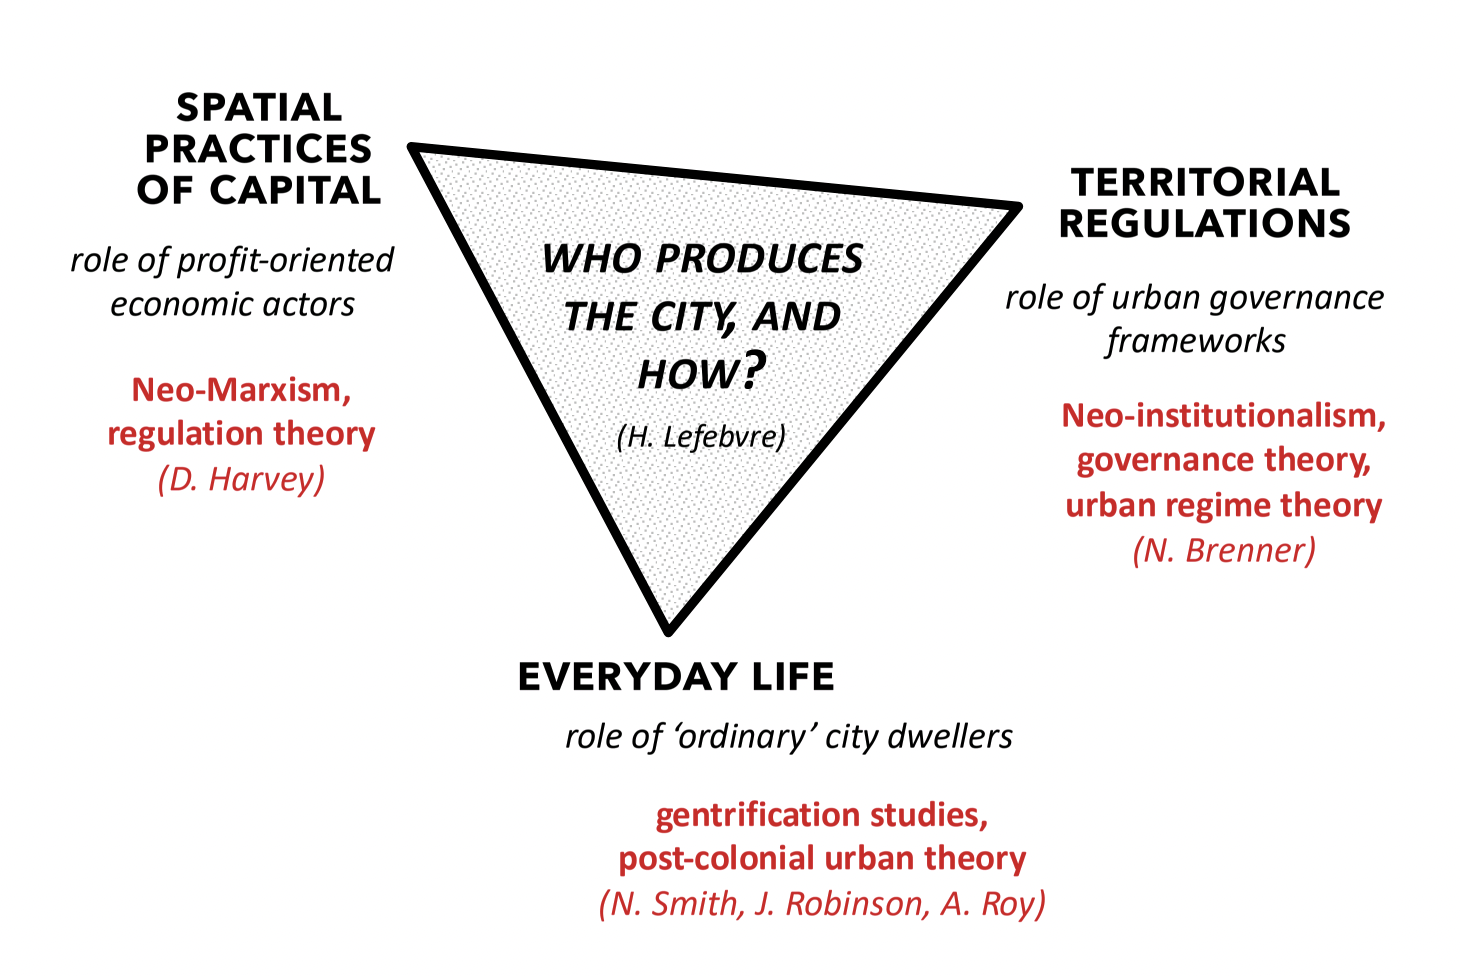
\includegraphics[width=\textwidth]{map_course_organisation1}
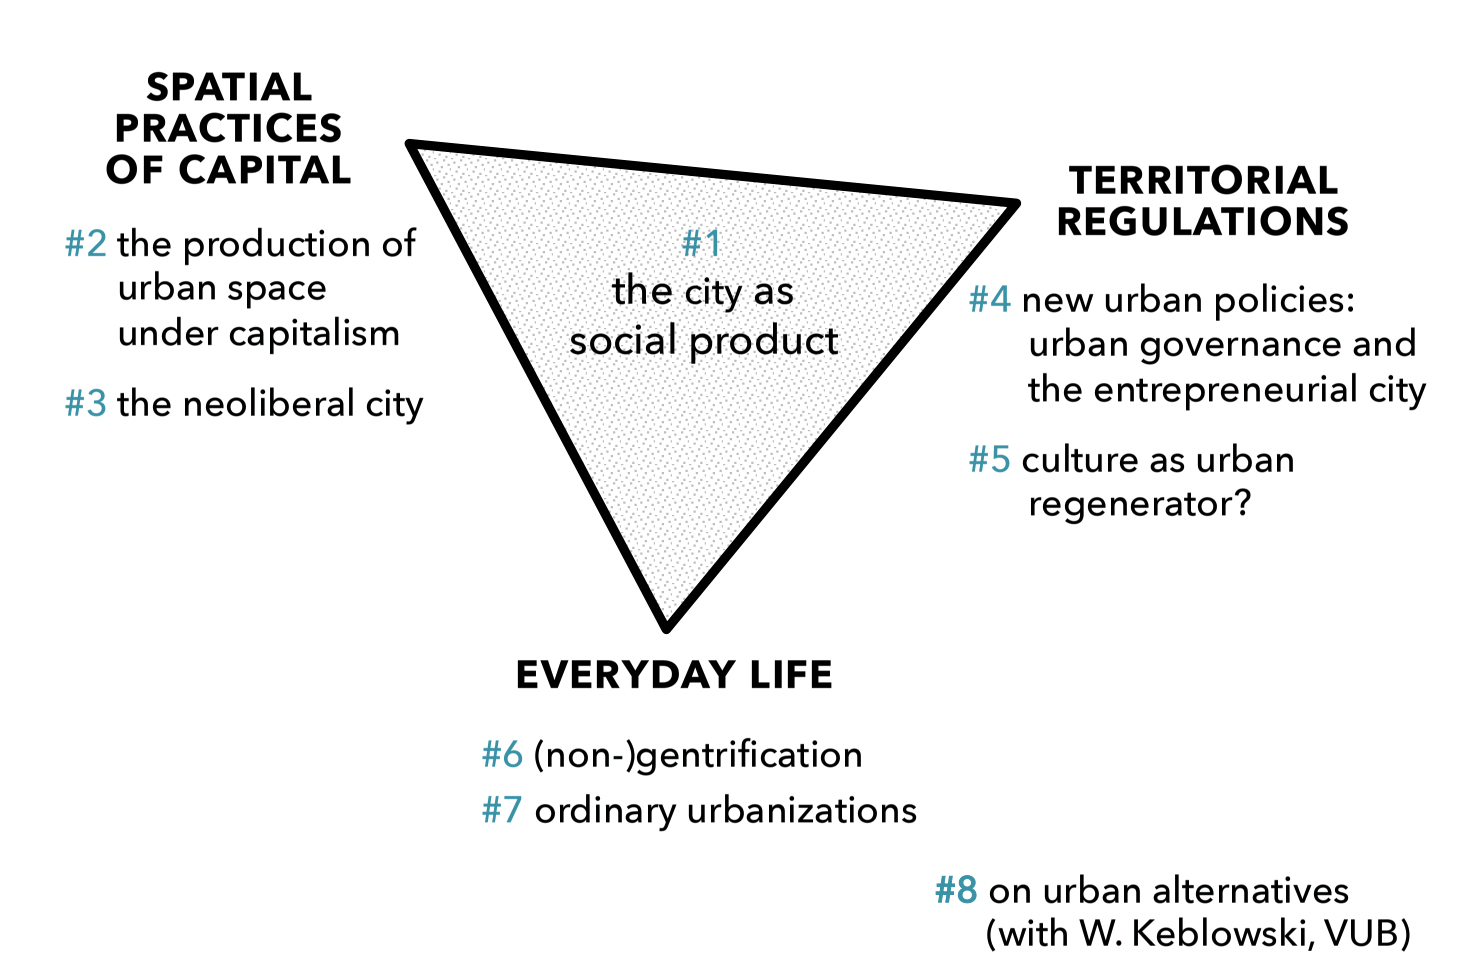
\includegraphics[width=\textwidth]{map_course_organisation2}

% LECTURE 2

\section{The Production of Urban Space Under Capitalism}

\section{The Neoliberal City}

\section{New Urban Policies: Urban Governance and the Entrepreneurial City}

\section{Culture as Urban Regenerator?}

\section{(Non-) Gentrification}

\section{Ordinary Urbanizations}

\section{On Urban Alternatives}

\end{document}